\documentclass[xcolor]{beamer}

% Pacotes Principais -----------------------------------------------------------
\usepackage[portuges,brazil]{babel}
\usepackage[utf8]{inputenc}

% Formatação de capítulos ------------------------------------------------------
%\usepackage[Sonny]{fncychap}
%\usepackage{fncychap}
\usepackage{capitulos}

% Figuras e Imagens ------------------------------------------------------------
\usepackage{graphicx}
% Figuras lado a lado
\usepackage{epsfig}
\usepackage{subfigure}

% Utilizar H para inserir as imagens REALMENTE onde eu desejo
\usepackage{float}

% Fontes -----------------------------------------------------------------------
\usepackage[T1]{fontenc}
\usepackage{pslatex}

% Simbolos ---------------------------------------------------------------------
\usepackage{textcomp}
\usepackage{bbding}

% Tabelas ----------------------------------------------------------------------
%\usepackage{multicol}
\usepackage{multirow}
% Colorir a tabela
\usepackage{colortbl}
% Pacote hhline corrige os bugs das linhas que não aparecem com o colortbm
\usepackage{hhline}
% Tabelas com colunas de largura auto ajustável
\usepackage{tabularx}
% Notas de rodapé em tabelas (Pode-se usar o ambiente longtable também -
% Pesquisar exemplo com longtable)
\usepackage{threeparttable}
% Tabelas grandes
\usepackage{supertabular}

% Glossário --------------------------------------------------------------------
\usepackage[portuguese,noprefix]{nomencl}
\usepackage{makeglo}

% Outros pacotes ---------------------------------------------------------------
\usepackage{noitemsep}

% Comentários em bloco
\usepackage{verbatim}

% Hiperlinks
\usepackage{hyperref}

% Orientação de página
\usepackage{lscape}

% utilitários matemáticos
\usepackage{amsmath}
\usepackage{icomma}

% Evita o problema "too many unprocessed floats", colocando os campos
% 'flutuantes' em suas respectivas seções
\usepackage[section]{placeins}

% Referências ------------------------------------------------------------------
\usepackage[abbr]{harvard}	% As chamadas são sempre abreviadas
\harvardparenthesis{square}	% Colchetes nas chamadas
\harvardyearparenthesis{round}	% Parêntesis nos anos das referências
\renewcommand{\harvardand}{e}	% Substituir "&" por "e" nas referências

% Comandos gerais --------------------------------------------------------------
\newcommand{\titulo}{Sistemas de Tempo Real}
\newcommand{\autor}{Diogo Leite Rebouças}

% Configuração da fonte
%\renewcommand{\familydefault}{\sfdefault}

% Margens ----------------------------------------------------------------------
\setlength{\oddsidemargin}{3.5cm}
\setlength{\evensidemargin}{2.5cm}
\setlength{\textwidth}{15cm}
\addtolength{\oddsidemargin}{-1in}
\addtolength{\evensidemargin}{-1in}

\setlength{\topmargin}{2.0cm}
\setlength{\headheight}{1.0cm}
\setlength{\headsep}{1.0cm}
\setlength{\textheight}{22.7cm}
\setlength{\footskip}{1.0cm}
\addtolength{\topmargin}{-1in}

% Glossário --------------------------------------------------------------------
\makeglossary

% Capítulos --------------------------------------------------------------------
% Não aparecer o número na primeira página dos capítulos
\newcommand{\mychapter}[1]{\chapter{#1}\thispagestyle{empty}}
\newcommand{\mychapterstar}[1]{\chapter*{#1}\thispagestyle{empty}}

% Comandos matemáticos ---------------------------------------------------------
% Implicação em fórmulas
\newcommand{\implica}{\quad\Rightarrow\quad} %Meio de linha
\newcommand{\implicafim}{\quad\Rightarrow}   %Fim de linha
\newcommand{\tende}{\rightarrow}

% Fração com parenteses
\newcommand{\pfrac}[2]{\parent{\frac{#1}{#2}}}

% Transformada de Laplace e transformada Z
\newcommand{\lapl}{\pounds}
\newcommand{\transfz}{\mathcal{Z}}

% Sequências
\newcommand{\sequencia}[4]{$#1_{#2}$, $#1_{#3}$, \ldots, $#1_{#4}$}

% Outros ----------------------------------------------------------------------
\newcommand{\chave}[1]{\left\{#1\right\}}
\newcommand{\colchete}[1]{\left[#1\right]}
\newcommand{\parent}[1]{\left(#1\right)}

\newcommand{\rhoagua}{\rho_{\tiny \text{\tiny H}_2\text{\tiny O}}}

\let\D\displaystyle
\newcommand{\reg}{\textsuperscript{\textregistered}}
\newcommand{\soft}{\textit{software}}
\newcommand{\Soft}{\textit{Software}}

% Imagens exportadas pelo gnuplot ----------------------------------------------
\graphicspath{{imgs/eps/}}


% Temas ========================================================================
\mode<presentation>
{
%\usetheme[blue,noshadow]{Trondheim}
%\usetheme[blue,minimal]{Trondheim}
\usetheme[blue,compress,numbers,nonav]{Trondheim}
%\usetheme[sand,compress,numbers,nonav,innovation]{Trondheim}
%\usetheme{default}

% Inner ........................................................................
%\useinnertheme{default}
%\useinnertheme{rounded}
%\useinnertheme{inmargin}
%\useinnertheme{rectangles}
\useinnertheme{circles}

% Outer ........................................................................
%\useoutertheme{default}
%\useoutertheme{infolines}
%\useoutertheme{miniframes}
%\useoutertheme{ntnu}
%\useoutertheme{shadow}
%\useoutertheme{sidebar}
%\useoutertheme{smoothbars}
%\useoutertheme{smoothtree}
%\useoutertheme{split}
%\useoutertheme{tree}

% Color ........................................................................
%\usecolortheme{albatross}
%\usecolortheme{beaver}
%\usecolortheme{beetle}
%\usecolortheme{crane}
%\usecolortheme{default}
%\usecolortheme{dolphin}
%\usecolortheme{dove}
%\usecolortheme{fly}
%\usecolortheme{lily}
%\usecolortheme{ntnublue}
%\usecolortheme{ntnuold}
%\usecolortheme{orchid}
%\usecolortheme{rose}
%\usecolortheme{seagull}
%\usecolortheme{seahorse}
%\usecolortheme{sidebartab}
%\usecolortheme{structure}
%\usecolortheme{whale}
%\usecolortheme{wolverine}
}

% Configuração da página inicial ===============================================
\title[Sistemas Multimídia]
{
    Sistemas Multimídia
}
\subtitle{Noções fundamentais de Sistemas Multimídia}
\author[Diogo Leite Rebouças]
{
    Diogo Leite Rebouças\\
    {\tt diogolr@gmail.com}
}
\institute
{
    Universidade do Estado do Rio Grande do Norte\\
    Departamento de Informática
}
\date{\today}
\pgfdeclareimage[width=1.5cm,interpolate=true]{ntnulogotext}{imgs/uern}

% Inicio do documento ==========================================================
\begin{document}

\maketitle
%\compressedtitle

% Logo somente após a capa
\logo{
\includegraphics[width=0.75cm]{imgs/uern}}

% Sumário ......................................................................
\begin{frame}
    \frametitle{Sumário}
    \tableofcontents
\end{frame}

\section{Introdução}
\subsection{O que é multimídia?}
\begin{frame}
    \frametitle{O que é multimídia?}
    
    Quando pessoas distintas mencionam o termo {\bf multimídia} talvez
    estejam querendo coisa também diferentes:

    \begin{itemize}
        \item Um \alert{vendedor de computadores}: Computador que possui som,
drive de DVD, processadores gráficos dedicados ou até que possui instruções de
máquina específicas para processar dados multimídia
        \item Um \alert{vendedor de entretenimentos}: Interatividade com a TV a
Cabo, que possui centenas de canais disponíveis ou Internet a cabo
        \item Um \alert{estudante de ciências da computação}: Aplicações que
fazem uso de múltiplos recursos (texto, vídeo, imagens, desenhos, animações,
som, fala, interatividade \ldots )
    \end{itemize}

    Multimídia + Ciências da Computação:

    \begin{itemize}
        \item Gráficos, IHC, visualização, visão computacional, compressão de
dados, comunicação, sistemas de banco de dados \ldots
    \end{itemize}

\end{frame}

\subsection{Elementos dos SM}
\begin{frame}
    \frametitle{Elementos dos SM}
    
    Aplicações Multimídia envolvem diversas ``modalidades'' e recursos
computacionais

    \begin{itemize}
        \item Texto
        \item Vídeo
        \item Áudio
        \item Desenhos
        \item Animações
    \end{itemize}

    Exemplos:

    \begin{itemize}
        \item Videoconferência
        \item Tele-medicina
        \item Ambientes de trabalhos cooperativos
        \item Realidade Virtual Aumentada
    \end{itemize}
\end{frame}

\subsection{Pesquisas na área}
\begin{frame}
    \frametitle{Pesquisas}

    Diversas áreas de atuação:

    \begin{itemize}
        \item \alert{Codificação e processamento multimídia}: análise de
conteúdo, recuperação de informações, segurança multimídia, processamento de
áudio/imagem/vídeo, compressão etc.
        \item \alert{Comunicação e suporte multimídia}: protocolos de rede,
internet, sistemas operacionais, clientes e servidores, qualidade de serviço
(QoS) e banco de dados
        \item \alert{Ferramentas multimídia e sistemas dedicados}: sistemas
hipermídia, interfaces de usuário
        \item \alert{Interação e integração multi-modais}: dispositivos móveis
com internet, educação multimídia (ensino colaborativo com auxílio do
computador), design e aplicações de realidade virtual
    \end{itemize}
\end{frame}

\begin{frame}
    \frametitle{Pesquisas}

    Tópicos mais pesquisados atualmente:

    \begin{itemize}
        \item \alert{{\it Tracking} de objetos}: movimentação da câmera baseada
em objetos-referência
        \item \alert{Captura de movimentos 3D}: modelos virtuais com movimentos
realísticos baseados em múltiplos atores reais (Avatar)
        \item \alert{Visões múltiplas}: sintetização de atores virtuais a partir
de múltiplas câmeras ou de câmeras únicas com iluminação diferencial
        \item \alert{Aplicações especializadas}: pessoas com visão comprometida
ou idosos
        \item \alert{Sistemas de monitoramento residencial}: dispositivos para
monitoramento da saúde das pessoas em uma residência (infarto)
    \end{itemize}
\end{frame}

\subsection{Aspectos históricos}
\begin{frame}
    \frametitle{Aspectos históricos}

    História da multimídia:

    \begin{itemize}
        \item Jornais: talvez seja o primeiro meio de comunicação em massa que
utilizava texto, imagem e gráfico
        \item Imagens em movimento: utilizadas por volta de 1830 para analisar a
rapidez de percepção do olho humano
        \item Transmissão sem fio (rádio): Primeira vez em 1895 na Itália
(Guglielmo Marconi)
        \item Televisão: novo meio de comunicação do século XX, estabeleceu o
vídeo como ``meio padrão'', mudando os conceitos sobre comunicação em massa
    \end{itemize}
\end{frame}

\begin{frame}
    \frametitle{Aspectos históricos}

    \begin{itemize}
        \item Comunicação entre computadores \implica período curto:

        \begin{itemize}
            \item 1945: primeiro artigo de referência sobre um sistema
hipermídia (Memex)
            \item 1960: início da utilização do termo {\bf hipertexto}
            \item 1969: primeiro editor hipertexto (FRESS)
            \item 1989: proposição da {\it World Wide Web} (WWW) por Tim
Berners-Lee
            \item 1991: aprovação do padrão de vídeo digital MPEG-1 \implica
levou a novos padrões MPEG-2, MPEG-4 dentre outros
            \item 1992: JPEG como padrão internacional de compressão de imagens
        \end{itemize}
    \end{itemize}
\end{frame}

\begin{frame}
    \frametitle{Aspectos históricos}

    \begin{itemize}
        \item Continuação \ldots
        \begin{itemize}
            \item 1994: criação do {\it Netscape}
            \item 1995: criação da linguagem {\it Java} para desenvolvimento de
aplicações ``independentes de plataforma''
            \item 1996: introdução dos vídeos em DVD \implica filmes de ``alta
qualidade'' distribuídos em uma única mídia
            \item 1998: anúncio do {\it XML 1.0}
            \item 1998: dispositivos móveis mp3 (32 MB de memória flash)
            \item 2000: estimativa de mais de 1 bilhão de sites na WWW
            \item Década de 2000: novos algoritmos de compressão, vídeos em alta
resolução, tv digital, disseminação das mídias, vídeos por demanda, \it
streaming de vídeo
        \end{itemize}
    \end{itemize}
\end{frame}

\section{Multimídia}
\subsection{Conceitos fundamentais}
\begin{frame}
    \frametitle{Conceitos fundamentais}

    \defin{Multimídia são todos os programas e sistemas em que a comunicação
entre homem e computador se dá através de múltiplos meios de representação de
informação (som, imagem, animações).}

    A multimídia requer:

    \begin{itemize}
        \item {\bf Acesso não linear:} Informação rapidamente acessível, não há
sequência de tempo como uma leitura de um livro, uma palestra ou um filme
        \item {\bf Interatividade:} Usuário como participante de uma atividade
computacional
        \item {\bf Integração inter-aplicativos:} Sistema de gestão de estoque +
Banco de Dados
    \end{itemize}
\end{frame}

\begin{frame}
    \frametitle{Conceitos fundamentais}

    As mesmas técnicas utilizadas para a criação multimídia podem ser usadas na
produção de mídias convencionais 

    \vspace{0.25cm}

Nem sempre o computador é a forma mais adequada para se apresentar a informação
(custo, aplicabilidade \ldots)

    \vspace{0.25cm}

    A criação de imagens, vídeos ou sons na forma digital traz benefícios mesmo
quando o produto final for distribuído em mídia analógica
\end{frame}

\subsection{Evolução da comunicação}

\begin{frame}
    \frametitle{Evolução da comunicação}

    Digitalização da informação:

    \begin{itemize}
        \item Computadores passaram a ser capazes de atender (suprir) as
necessidades dos grandes fluxos de dados (informação)
        \item Aplicações hoje \implica Telefonia fixa, móvel, TV, vídeos, foto,
cinema, {\it players} portáteis, termômetros \ldots
    \end{itemize}

    Ambientes textuais:

    \begin{itemize}
        \item Computadores primitivos funcionavam quase como uma máquina de
escrever \implica Algumas aplicações hoje ainda utilizam essa ideia
(interpretadores de comandos DOS, Unix) \implica Aplicativos orientados para
linhas (40 a 80 caracteres -- {\bf unidades de interação})
        \item Surgimento dos terminais alfanuméricos de raios catódicos \implica
Aplicativos orientados a tela (1000 a 3000 caracteres) \implica Semelhante aos
processadores de texto \implica Exemplos: Wordstar e Vi
    \end{itemize}
\end{frame}

\begin{frame}
    \frametitle{Conceitos fundamentais}
    
    Ambientes gráficos:

    \begin{itemize}
        \item Aplicações passaram a ser orientadas (endereçáveis) por pontos
({\it pixes})
        \item Alto custo inicial \implica Utilização somente para aplicações em
que o processamento gráfico era essencial: ambientes CAD, automação industrial
\ldots
        \item Surgimento dos sistemas operacionais baseados em Janelas
(RWindow\$, Linux)
        \item Processadores de texto ganham versões {\it WYSIWYG}
    \end{itemize}
\end{frame}

\subsection{Ambientes multimídia}
\begin{frame}
    \frametitle{Ambientes multimídia}

    O que se aplica:

    \begin{itemize}
        \item Emprego de animação: Necessidade de taxa mínima de atualização da
tela
        \item Emprego do som: Ouvido humano é extremamente sensível a
pequenas deformações temporais do som \implica Maior preocupação com relação a
reprodução (diferentemente da imagem)
        \item Substituição de mídias convencionais: Maior flexibilidade
para criação de mídias visuais e sonoras \implica Possibilidade de combinação de
mídias digitais com mídias analógicas
        \item Produtos multimídia: Utilizados para permitir ao usuário
diferentes graus de interação
    \end{itemize}
\end{frame}

\begin{frame}
    \frametitle{Ambientes multimídia}

    Interações do usuário através dos produtos multimídia:

    \begin{itemize}
        \item Percorrer material audiovisual de forma não-linear
        \item Consultar, pesquisar e atualizar conteúdo armazenado em bases de
dados audiovisuais
        \item Criar material audiovisual em tempo real a partir de modelos
cliente-servidor (solicitação-resposta) ou dados de instrumentos físicos ({\it
webcam})
        \item Simular sistemas físicos com diferentes graus de realismo
    \end{itemize}
\end{frame}

\begin{frame}
    \frametitle{Ambientes multimídia}

    Tipos de produtos\footnote{Entendam por produtos aquilo que é produzido}
multimídia (classificação por grau de interatividade):

    \begin{itemize}
        \item Títulos
        \item Aplicativos
        \item Sítios
    \end{itemize}

    \uline{\bf Títulos}

    \begin{itemize}
        \item Grau de comportamento rígido
        \item Se comportam mais como documentos do que como programas
        \item Flexibilidade embutida nos visualizadores ({\it viewers}) ou
navegadores ({\it browsers}) -- meios de consulta e pesquisa.
        \item Podem ser classificados em títulos lineares ou títulos hipermídia
    \end{itemize}

\end{frame}

\begin{frame}
    \frametitle{Ambientes multimídia}

    Títulos lineares $\times$ títulos hipermídia

    \begin{itemize}
        \item Títulos lineares

        \begin{itemize}
            \item Segue ordem pré-determinada e sequencial
            \item Exemplos: apresentações (palestras -- não confundir com {\it
slides}), demonstrações de produtos, apresentações em vídeo \ldots
        \end{itemize}

        \item Títulos hipermídia

        \begin{itemize}
            \item Derivam do conceito de hipertexto acrescido de imagem, sons e
animações
            \item Ordem de visualização determinada pelo usuário final através
de {\bf controles} para {\bf navegação não-sequencial}
            \item Controles: Indicações normalmente visuais (sinais gráficos),
tais como textos sublinhados, botões \ldots
            \item Exemplos: títulos de referência (dicionários, enciclopédias,
manuais de instrução), quiosques informativos (aeroporto), catálogos de produtos
e serviços
        \end{itemize}
    \end{itemize}

\end{frame}


\begin{frame}
    \frametitle{Ambientes multimídia}

\begin{figure}[htb]
\centering
\subfigure[Título linear]
{
    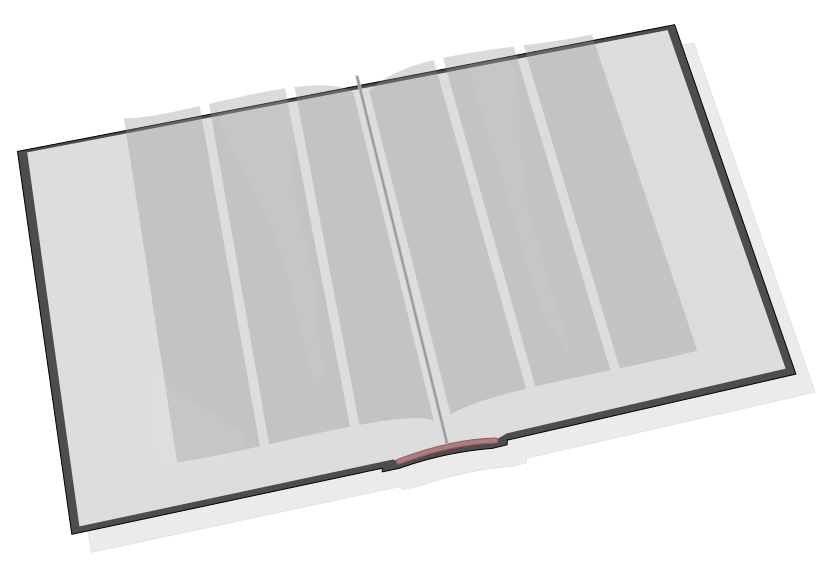
\includegraphics[width=0.45\textwidth]{imgs/livro}
}
\subfigure[Título hipermídia]
{
    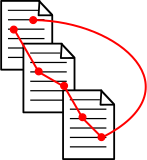
\includegraphics[width=0.35\textwidth]{imgs/texto}
}
\end{figure}
\end{frame}


\begin{frame}
    \frametitle{Ambientes multimídia}

    \uline{\bf Aplicativos}

    \vspace{0.25cm}

    Aplicativos com interface multimídia: 

    \begin{itemize}
        \item Desenvolvidos em ambientes de programação
        \item Utilizam recursos gráficos (Qt, Java, Python \ldots) e sonoros
para interagir com o usuário
        \item Exemplos: aplicativos convencionais, jogos, aplicativos
educacionais \ldots
    \end{itemize}

    Aplicativos multimídia:

    \begin{itemize}
        \item Processam material multimídia (geralmente em tempo real)
        \item Multimídia deixa de ser um recurso de interface e passa a ser
objeto de processamento do aplicativo
        \item Exemplos: ferramentas multimídia (produção de imagens, vídeos,
sons), simuladores de tempo real (automotivos, de aeronaves), sistemas de
informação geográfica \ldots
    \end{itemize}
\end{frame}

\begin{frame}
    \frametitle{Ambientes multimídia}

    \uline{\bf Sítios}

    Multimídia na internet:

    \begin{itemize}
        \item Possibilidade de acesso à informação de todo o mundo utilizando
``poucos recursos'' de {\it hardware} e {\it software}
        \item {\it World Wide Web} (WWW) como serviço hipermídia na internet
    \end{itemize}
        
    \defin{Sítio ({\it site}): {\bf Hipermídia} armazenada em um servidor WWW
que pode ser {\bf visualizado remotamente} (máquina cliente) através de um
programa (navegador). Os sítios são  {\bf \alert{normalmente} escritos em HTML}
({\it Hypertext Markup Language}) e a navegação se dá através de {\bf
hiperligações} ({\it hiperlinks}). {\bf Podem conter material multimídia}
(utilização de {\it plugins})}
\end{frame}

\end{document}
